





%%%%%%%%%%%%%%%%%%%%%%%%%%%%%%%%%%%%%%%%%%%%%%%%
%%%%%%%%%%%   Other Models   %%%%%%%%%%%%%%%%%%%
%%%%%%%%%%%%%%%%%%%%%%%%%%%%%%%%%%%%%%%%%%%%%%%%%


\hrule\vspace{1pt}\hrule
\begin{center}
\mbox{{\bf What Do We Expect?}} \\
\vspace{0.5em}
\mbox{{-----}}
\end{center}
\hrule




\section{Even More}

\paragraph{GOAL} Our task is to check if the method can be applied to $\Lambda$CDM, sCDM, $f(R)$, $\omega(z)$, DGP, CPL and interacting model\footnote{This might be only possible for $Q=sim\rho_{de}$}, using the DE model as an fiducial model.

The ultimate purpose is to get the matter power spectrum today, or to find constrain on the parameters of different models or even to rule out models.

And other purposes?



\subsection{FAQ}
\begin{enumerate}

\item Why we use both growth factor and transfer function to discribe the evolution of the power sepctrum?

If we try to inspect the potentials that stays outside of the horizon, we can find that those potentials changes the amplitude by 10\% during equality though they stay unchange both in radiation and matter epochs. This tells us that something special happened during equality. Thus we have to find a function to discribe this dropdown during equality, which is called transfer fucntion.

(An alternate view is given below.)
If the perturbations reenter at MD, the power spectrum $P(k,t)\propto C(t)k$. But it would be $P(k,t)\propto C(t)k^{-3}$ if the perturbations reenter at RD. These differences are caused by the different evolution of scale factor $a(t)$ during MD and RD. However, the universe dosen't transit from RD to MD suddenly. So if we want to write a unified equation of the power spectrum, it should be $P(k,t)\propto kT^2(k)D^2(t)$. The factor $T^(k)$ (it is the transfer func. actually) should transit from $k^{-3}/k$ in RD to $k/k$ in MD gradually. We can see that the transfer function is of unit during MD.

{\bf\color{red}More info. (including a Sokes-Navier view of the perturbation theory) is given in the {\it Cosmology Projects} notebook.}

\item When did the equality happen?

This can be calculated with the Friedmann equations if only we use the total density. Anyway, the answer to this is
\begin{equation}
\tau_{eq}=\frac{2(\sqrt 2 -1)c}{H_0}\sqrt{\frac{a_{eq}}{\Omega_m}}
\end{equation}
Conformal time is used here.{\bf\color{red} This function is useless because $a_{eq}$ is still unknown. }

\item
What about the transfer fucntion?

There are many forms of transfer functions, for example, the BBKS (Bardeen, Bond, Kaiser, and Szalay, 1986) one reads
\begin{eqnarray}
T^2(k)=\frac{\ln{(1+2.34q)}}{2.34q}\bigg[ 1+3.89q+(16.1q)^2+(5.46q)^3+(6.71q)^4 \bigg]^{-1/4}
\end{eqnarray}
in which, $q=k/\Gamma$ and $\Gamma=\Omega_Mh$.
There are also more accurate formulae. (Daniel J. Eisenstein and Wayne Hu, 1998, {\it Baryonic Features in The Matter Transfer Function.})

{\bf\color{red} How is it dealed with in their paper? Check the part about factor $Q$ in \ref{TransferFunctionSame}.}

\item
Growth Factor? What is growth factor by Scott Dodelson? Does it change the spectrum of early time?

The growth factor is defined as the collective growth ($k$ independent growth) of the perturbations in sub-horizon during MD (large $a/a_{eq}$ limit or large $a$ limit of extended Meszaros equation).

The equation for the perturbation of matter is 
{\footnote{
A different method from Scott and Ivan etc given by George at CalTec is to use the Stoke-Navier equaiton for continuous matter. Define $\delta_m$ as the perturbation of $\rho_m$ and drop the second and higher orders,
\begin{eqnarray}
\frac{\partial \delta_m}{\partial t}&=&-a^{-1}\nabla\cdot \vec v_m \\
\frac{\partial\vec v}{\partial t}&=&-\frac{\nabla \Phi}{a}-H\vec{ v_m} \\
a^{-2}\nabla^2\Phi&=&4\pi G \bar\rho_m\delta_m    .
\end{eqnarray}
Meanings of these eqns. are given in {\it Cosmology Projects} notebook.
}}
\begin{eqnarray}
\ddot \delta_m + 2H\dot \delta_m - 4\pi G \bar \rho_m \delta_m=0
\end{eqnarray}
It is a secondary ODE. So two linear indepent special solutions can be found. One mode stands for the growing of the perturbations and it is called the growth func., i.e., $\delta_m=C_1D_1(t)+C_2 D_2(t)$ and $D_2(t)\rightarrow 0$ at $t\rightarrow \infty$.

Sometimes growth rate ($f(a)=\mathrm d \ln{G(a)}/\mathrm d\ln a$) is used (because it is convinient to be shown in a logarithmatic figure, I think).

Since we would like to find the solution to $\delta_m$ to $a$, Scott rewrite the Meszaros equation
\begin{equation}
\frac{\mathrm d^2\delta}{\mathrm d a^2}+(\frac{\mathrm d \ln H}{\mathrm d a}+\frac{3}{a})\frac{\mathrm d \delta}{\mathrm d a}-\frac{3\Omega_m H_0^2}{2a^5 H^2}\delta=0    .
\end{equation}
We have a routine to solve such second order equations. ({\it Cosmology Projects} notebook)

The growing mode is
\begin{equation}
\delta\propto H(a)\int^a \frac{\mathrm d \tilde{a}}{(\tilde a H(\tilde a))^3}
\end{equation}

Equivalently, 
\begin{equation}
D_+(a)=\frac{5\Omega_m}{2}\frac{H(a)}{H_0}\int^a_0 \frac{\mathrm d \tilde{a}}{(\tilde a H(\tilde a)/H_0)^3}  .
\end{equation}



\item
What is the Hubble function?
\paragraph{For dark energy model} 
From the Friedmann equation, 
\begin{eqnarray}
\ddot a/a&=&-4/3\pi G(\rho+3p) \\
\dot \rho&=&-3\dot a/a(\rho+p)
\end{eqnarray}
for any state equation $w=p/\rho$ (in which $w$ is time independent), we have 
\begin{eqnarray}
\rho\cdot a^{3(1+w)}=\text{Const}=\rho_0 a_0^{3(1+w)}=C_1.
\end{eqnarray}

(Though it is easy to move on, we need nothing more.)
\footnote{Deform the second derivaive of $a$, 
\begin{eqnarray}
\ddot a&=&-\frac 4 3 \pi G \rho a (1+w) \\
&=&-\frac 4 3 \pi G \rho a^{3(1+w)}\frac{a}{a^{3(1+w)}} (1+3w) \\
&=&-\frac 4 3 \pi G (1+3w) C_1 a^{1-3(1+w)} \\
&=&C_2 a^{1-3(1+w)}
\end{eqnarray}

To solve that equation, we have to denote $y=\dot a$, then the second derivative of scale factor $a$ goes $\ddot a=y \frac{\mathrm d y}{\mathrm d a}$, the former equation becomes
\begin{eqnarray}
&&y\frac{\mathrm d y}{\mathrm da}=C_2a^{1-3(1+w)}\\
\rightarrow && \mathrm d (\frac 1 2 y^2)= C_2 \frac 1 {2-3(1+w)} \mathrm d a^{2-3(1+w)} \\
\rightarrow && \frac 1 2 y^2=C_3a^{2-3(1+w)}+C_4 \\
\rightarrow && y=\sqrt{ 2C_3 a^{2-3(1+w)} +2 C_4 }
\end{eqnarray}
																			
The hardest task is to determine how does scale factor $a$ evolve, i.e., solving the equation of $y$.

Actually this problem is a sole task of finding the initial states.}


Then Hubble function is
\begin{equation}
H^2=H_0^2[\Omega_{M0}(1+z)^3+\Omega_{R0}(1+z)^4+\Omega_{K0}(1+z)^2+\Omega_{DE0}(1+z)^{3(1+w)}]  \label{HubbleFunction} ,
\end{equation}
in which, $\Omega_{x0}=8\pi G \rho_{x0}/(3H_0^2)$ and 0 subscript stands for the present value.

(For $\Lambda$CDM, substitute $w$ with -1.)









Consequently, we can write down the growth factor analytically,{\footnote{
There are things to be clearified. The first thing is that this is scaled based on $D_+=a$ during matter domination. The second one is is little complicated. This growth func. is derived with a $a\gg a_{eq}$. But here the intergration starts from 0. The actual integration should be divided into several parts, i.e., RD, MD etc. Here it is OK to integrate from 0 because we have set the evolution in RD to be the same and lasts much shorter than MD and the perturbation changes little (compared to the changes in MD) during RD, if the perturbations come into horizon during RD. But for those come into horizon during deep MD, the integration should start from the moment they enter. {\color{red}Check what have been done in their paper. {\bf Also, it is important to check how the approximation for those entered in RD changes the final result.}}
}}
\begin{equation}
D_+(a)=\frac 5 2\Omega_m  \mathscr H(a)\int^a_0 \frac {1} {(\tilde a \mathscr H (\tilde a))^3} \mathrm d\tilde a     ,
\end{equation}
in which, $\mathscr H(a)^2=\Omega_{M0}a^{-3}+\Omega_{R0}a^{-4}+\Omega_{K0}a^{-2}+\Omega_{DE0}a^{-3(1+w)}$.





\item Why is there a $\sigma_8$?

Observations on present abundance of rich clusters of galaxies can only give constrains on $\sigma_8 \Omega$.{\footnote{
There are ways to break the degeneracy. Read astro-ph/9706018 for an example.
}}
$\sigma_8$ stands for the normalization of the power spectrum on $8h^{-1}$Mpc scale.

\end{enumerate}















\subsection{Models}
\subsubsection{sCDM Model}

In this model, our universe is dominated by matter (including baryons and dark matter) today {\footnote{
At late time of sCDM model, it becomes an Einstein-de Sitter model. This part (EdS) describes the real universe from $z\sim 1000$ to $z\sim 1$ very well.
}}. Typically, when the time is the power spectrum is given by
\begin{equation}
P(k,a)=2\pi^2\delta_H^2\frac{k^n}{H_0^{n+3}}T^2(k)\bigg(\frac{D_1(a)}{D_1(a=1)}\bigg)^2
\end{equation}


\begin{itemize}

\item 
$\delta_H$ is the primordial horizon scale perturbation and we can set this to be the same in different models.

\item 
$H_0$ is the Hubble constant today.

\item
We can just set $n=1$ for Zeldovich spectrum since we are not requiring a very accruate calculation.

\end{itemize}




If we want to calculate the accurate power of the matter perturbations, we have to get $T$ and $D_1$.

However, we will just calculate the growth factor now. 
In {\bf flat sCDM model, i.e., EdS model}, $\Omega_M(a)=\Omega_{M0}=1$, $\Omega_{K0}=\Omega_{R0}=\Omega+_{DE0}=0$ ($\mathscr H=a^{-3}$ by applying \ref{HubbleFunction}). Then the growth factor is
\begin{eqnarray}
D_+(a)
&=&\frac 5 2 \cdot 1 \cdot a^{-3/2} \cdot \int^a_0 {\tilde a}^{-3/2}\mathrm d \tilde a   \\
&=&a
\end{eqnarray}






\subsubsection{$\Lambda$CDM}

Assume we have $\Omega_{M0}=n$, then $\Omega_{\Lambda 0}=1-n$ since other components dispear far after equality in a flat $\Lambda$CDM model.

Take $\Omega_{\Lambda 0}=0.7$ as an example.{\footnote{
Check the mathematica file to find out more.
}}



Two examples are calculated to show the difference.{\footnote{
They are normalised to the same value at $a=0.1$.
}}{\footnote{{\color{blue}These figures for growth factors are useless for our goal. I put them here to show they can be calculated.}{\color{red}However, these calculations are just toy models because I used a lot approximation here. Formal calculations can be done by using NIntegrate in mathematica.}}}

a. Red line is the growth factor of sCDM model while blue line is that of $\Lambda$CDM model.


\begin{figure}[h]

\centering
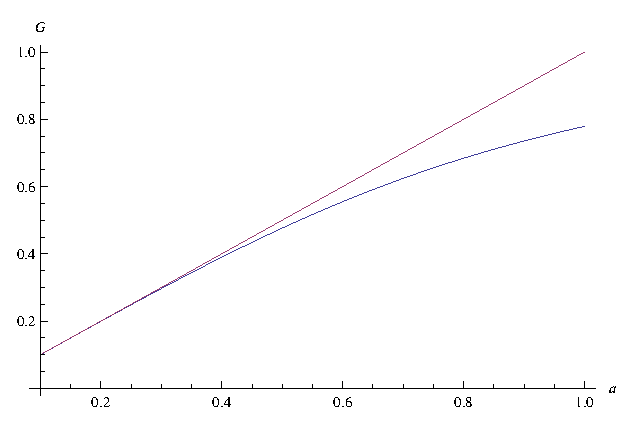
\includegraphics{P_sCDM+LCDM_G.eps}
\caption{Growth factors of sCDM and $\Lambda$CDM}
\end{figure}

\begin{figure}
\centering
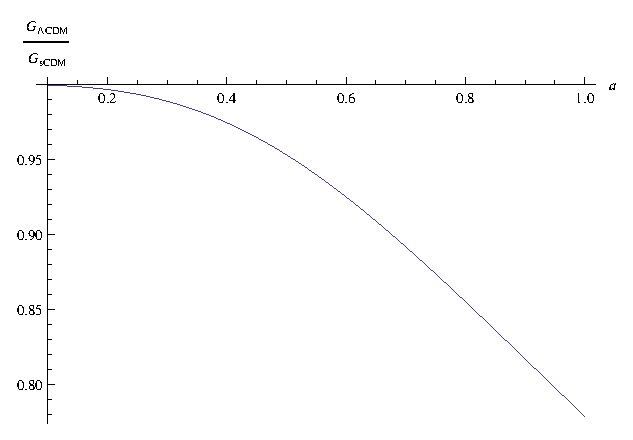
\includegraphics{P_sCDM+LCDM_G2.eps}
\caption{Ratio of the growth factors.($\Lambda$CDM to sCDM.)}
\end{figure}




\subsubsection{DE}

Similar calculations generate the growth factor for dark energy model (figure \ref{DE_G}) and the difference between sCDM and dark energy model(figure \ref{DE+sCDM_G}).{\footnote{{\color{red}
These are calculated using Mathematica. The mathematica notebook file is located in the same folder of the {\LaTeX} file. Brief notations are given in that file.
}}}

\begin{figure}[h]
\centering
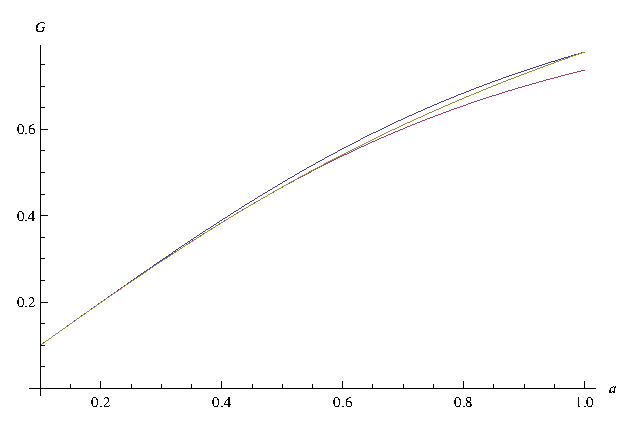
\includegraphics{P_DE_Growth.eps}
\caption{Growth factors of dark energy models with different EoS. The blue line,  red line and green line stand for $w=-0.9$, $w=-1.0$ (it reduces to $\Lambda$CDM model) and $w=-1.1$ respectively.} \label{DE_G}
\end{figure}

\begin{figure}[h]
\centering
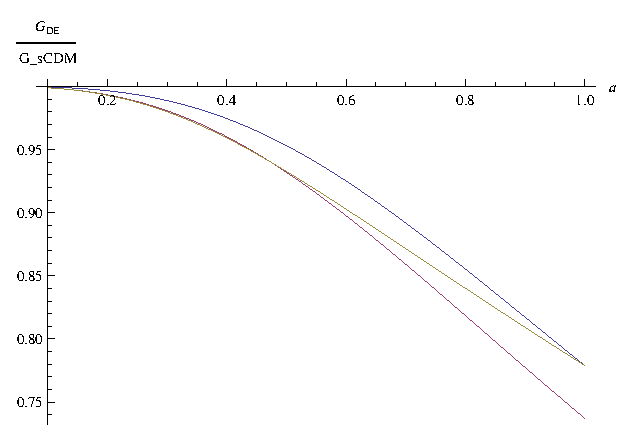
\includegraphics{P_DE+sCDM_G.eps}
\caption{The ratio of growth factors of dark energy model to that of sCDM model.The blue line,  red line and green line stand for $w=-0.9$, $w=-1.0$ (it reduces to $\Lambda$CDM model) and $w=-1.1$ respectively. }\label{DE+sCDM_G}
\end{figure}


\subsubsection{f(R)}
\subsubsection{DGP}
\subsubsection{CPL}
\subsubsection{Interacting?}




\subsection{Power Spectrum}

Calculate the power spectrum of a fiducial model using CMBEASY. {\color{red}I did a little calculation, but it seemed the data never went right. I will check this later.}




